%======================================================================
% L04b_Equilibrium.pdf
%======================================================================
% přeškrtnutí v rovnici (balík cancel není k dispozici)
\providecommand{\cancel}[1]{\tikz[baseline=(c.base)]{\node[inner sep=0pt](c){$#1$};\draw[NavyBlue](c.south west)--(c.north east);}}
\section{Podmínky rovnováhy a intenzivní parametry}
\strana{L04b-1}

\begin{itemize}
  \item \kw{Fundamentální rovnice v entropické reprezentaci}
  \[
    S = S(U, X_1,\dots,X_n) \ \xrightarrow{\text{spec.}}\ S = S(U,V,N) \qquad \textcolor{Red}{(P1,2)}
  \]
  \item \textcolor{Red}{(P3)} diferencovatelnost $\Rightarrow$ \quad
  $\dd S = \left(\pdv{S}{U}\right)_{V,N}\dd U + \left(\pdv{S}{V}\right)_{U,N}\dd V + \left(\pdv{S}{N}\right)_{U,V}\dd N$
\end{itemize}

\underline{Otázka:} \quad Význam $\left(\pdv{S}{X_i}\right)_{X_{j\neq i}} = \;?$

\begin{itemize}
  \item charakteristika rovnovážného stavu:
  \[
    \begin{aligned}
      \dd S &= 0 &&\Leftrightarrow\ \text{extrém -- rovnováha} \\
      \dd^2 S &< 0 &&\Leftrightarrow\ \text{maximum -- stabilita}
    \end{aligned}
    \qquad \textcolor{Red}{(P1,2,3)}
  \]
\end{itemize}

\subsection*{1) Tepelná rovnováha}
\hfill \textcolor{NavyBlue}{$S = S(\underbrace{U,V,N}_{\text{fix}};\ \underbrace{U_1,V_1,N_1}_{\text{volné}}) \xrightarrow{\ \max\ } S = S(U,V,N)$}

\[
  S = S_1(U_1,V_1,N_1) + S_2(U_2,V_2,N_2) \qquad \leftarrow \text{aditivita } \textcolor{Red}{(P4)}
\]

\underline{Pozn:}
\begin{itemize}[nosep]
  \item zde na jednu stranu zanedbáváme interakci, na druhou stranu ji potřebujeme pro realizaci tep.\ kontaktu; předp.\ tedy režim
  \[
    U_{\text{int}} \ll U_1 + U_2\,; \qquad \text{\uv{$S_{\text{int}}$}} \ll S_1 + S_2
  \]
  ($\Leftrightarrow$ příspěvek rozhraní $\ll$ příspěvek objemu)
\end{itemize}

\begin{itemize}
  \item $\dd V_i = 0$, \ $\dd N_i = 0$ \quad $\Rightarrow$ \quad 1) \
  $\dd S = \left(\pdv{S_1}{U_1}\right)_{V_1,N_1}\dd U_1 + \left(\pdv{S_2}{U_2}\right)_{V_2,N_2}\dd U_2 = 0$ \\
  \hspace*{6.4cm} i.e.\ $\dd U = \dd U_1 + \dd U_2 = 0$ \quad (ZZE)
\end{itemize}
\[
  \Rightarrow\quad \dd S = \left[\left(\pdv{S_1}{U_1}\right)_{V_1,N_1} - \left(\pdv{S_2}{U_2}\right)_{V_2,N_2}\right]\dd U_1 \equiv 0
\]
\[
  \Rightarrow\quad \left(\pdv{S_1}{U_1}\right)_{V_1,N_1} = \left(\pdv{S_2}{U_2}\right)_{V_2,N_2} \qquad \text{v rovnováze}
\]

\begin{veta}[Teplota]
$\Rightarrow\ \left(\pdv{S}{U}\right)_{V,N}$ \ má charakter teploty: \quad
\begin{tabular}[t]{l}
1) intenzivní veličina \\
2) stejná pro syst.\ v rovnováze
\end{tabular}
\end{veta}

%----------------------------------------------------------------------
\strana{L04b-2}
\begin{itemize}
  \item směřování do rovnováhy:
\end{itemize}
\[
  \dd S = \left[\left(\pdv{S_1}{U_1}\right)_{V_1,N_1} - \left(\pdv{S_2}{U_2}\right)_{V_2,N_2}\right]\dd U_1 > 0
\]
\textcolor{NavyBlue}{\small Podmínka rovnováhy je \
$\frac{1}{T_1}(U_1,V_1,N_1) = \frac{1}{T_2}(\underbrace{U - U_1}_{U_2}, V_2, N_2)$
\ $\Updownarrow$ \ rovnice pro $U_1 \Rightarrow S(U_1,V_1,N_1)$}
\[
  \Rightarrow\quad
  \begin{cases}
    \left(\pdv{S_1}{U_1}\right) > \left(\pdv{S_2}{U_2}\right) \ \Rightarrow\ \dd U_1 > 0 \ \Rightarrow\ \text{\uv{teplo} } 2\to 1 \\[6pt]
    \left(\pdv{S_1}{U_1}\right) < \left(\pdv{S_2}{U_2}\right) \ \Rightarrow\ \dd U_1 < 0 \ \Rightarrow\ Q\ \ 1\to 2
  \end{cases}
\]
$\Rightarrow$ \uv{teplejší} $\Leftrightarrow$ menší $\left(\pdv{S_i}{U_i}\right)$ \quad $\Rightarrow$ jako \uv{inverzní teplota}

\begin{definice}[Teplota]
$\Rightarrow$ definuji \qquad
$\vzorec{\dfrac{1}{T} \equiv \left(\pdv{S}{U}\right)_{\{X_i\}}}$
\qquad \dots\ definice samozřejmě konzistentní s původním odvozením:
\end{definice}
\[
  \dd S = \frac{1}{T}\dd U + \dots \ \Rightarrow\
  \Big/\left(\pdv{U}{S}\right)_X = \Big[\underbrace{\left(\pdv{S}{U}\right)_X}_{>0\ \textcolor{Red}{(P3)}}\Big]^{-1}\Big/
  \ \Rightarrow\ \dd U = T\,\dd S + \dots
\]

\subsection*{2) Mechanická rovnováha}

\begin{minipage}{0.45\textwidth}
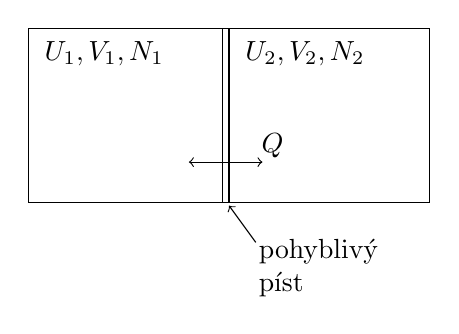
\begin{tikzpicture}[scale=0.85]
  \draw (0,0) rectangle (6,2.6);
  \draw (2.9,0) -- (2.9,2.6);
  \draw (3,0) -- (3,2.6);
  \node[anchor=north west] at (0.1,2.55) {$U_1,V_1,N_1$};
  \node[anchor=north west] at (3.1,2.55) {$U_2,V_2,N_2$};
  \draw[<->] (2.4,0.6) -- (3.5,0.6);
  \node at (3.65,0.85) {$Q$};
  \draw[->] (3.4,-0.6) -- (3,-0.05);
  \node[anchor=north west,align=left] at (3.3,-0.4) {pohyblivý\\píst};
\end{tikzpicture}
\end{minipage}
\begin{minipage}{0.53\textwidth}
\begin{enumerate}[label=\roman*),nosep]
  \item $\dd S = \sum_i\left[\left(\pdv{S_i}{U_i}\right)_{V_i,N_i}\dd U_i + \left(\pdv{S_i}{V_i}\right)_{U_i,N_i}\dd V_i\right] = 0$
  \item $\dd V_1 + \dd V_2 = 0$
  \item $\dd U_1 + \dd U_2 = 0$
\end{enumerate}
\medskip
\textcolor{NavyBlue}{\fbox{\parbox{4.5cm}{\underline{Pozn:} Co když se nevyměňuje teplo? \\ Viz cvičení}}}
\end{minipage}

\[
  \Rightarrow\quad
  \begin{aligned}
    &a)\quad \left(\pdv{S_1}{U_1}\right)_{V_1,N_1} = \left(\pdv{S_2}{U_2}\right)_{V_2,N_2}
      &&\Leftrightarrow\ \frac{1}{T_1} = \frac{1}{T_2} \\
    &b)\quad \left(\pdv{S_1}{V_1}\right)_{U_1,N_1} = \left(\pdv{S_2}{V_2}\right)_{U_2,N_2}
      &&\overset{\text{def.}}{\Leftrightarrow}\ \frac{p_1}{T_1} = \frac{p_2}{T_2} \ \Rightarrow\ p_1 = p_2
  \end{aligned}
\]
\textcolor{Red}{\small $T_i = T_i(U_i,V_i,N_i)$, $p_i = p_i(U_i,V_i,N_i)$ $\Rightarrow$ jedná se o rovnice pro rovnovážné $U_i, V_i$; + rovnice vazeb}

\begin{definice}[Tlak]
$\Rightarrow$ definuji \qquad
$\vzorec{\left(\pdv{S}{V}\right)_{U,N} \equiv \dfrac{p}{T}}$
\qquad $\Rightarrow$ \quad
$\begin{aligned}[t]
  \dd S &= \tfrac1T\dd U + \tfrac{p}{T}\dd V + \dots \\
  \dd U &= T\,\dd S - p\,\dd V + \dots
\end{aligned}$
\end{definice}

%----------------------------------------------------------------------
\strana{L04b-3}
\begin{itemize}
  \item směřování do rovnováhy:
\end{itemize}
\[
  \left[\left(\pdv{S_1}{V_1}\right) - \left(\pdv{S_2}{V_2}\right)\right]\dd V_1 > 0
  \ \Rightarrow\ \frac{p_1}{T_1} > \frac{p_2}{T_2}\ \Rightarrow\ \dd V_1 > 0
  \qquad \checkmark\ \text{\textcolor{NavyBlue}{\small znaménko u tlaku OK}}
\]
\textcolor{NavyBlue}{\small $\bullet$ že je to $\frac{p}{T}$ a ne \uv{$\pi$}: rozměr.\ analýza + intenzivita \
$[\pi] = \left[\frac{S}{V}\right] = [V^{-1}] \Rightarrow \dd S = \pi\,\dd V$ \& $\dd U = T\dd S\dots$}

\subsection*{Teplo vs.\ práce}
\begin{enumerate}[label=\arabic*)]
  \item dodáme do systému pouze \underline{teplo $\dd Q$} \textcolor{NavyBlue}{\small ($\Updownarrow$ extenzivní parametry se nemění)} \\
  $\Rightarrow$ i) $U\to U + \dd Q$; \quad $V,N = \text{konst.}$
  \[
    \Rightarrow\ \dd S = S(U + \dd Q, V, N) - S(U,V,N) = \left(\pdv{S}{U}\right)_{V,N}\dd Q = \frac{\dd Q}{T}
  \]

  \begin{minipage}{0.3\textwidth}
  \textcolor{NavyBlue}{\small \underline{Tedy} teplo je změna energie za konst.\ $X_i \Rightarrow \dd Q = T\dd S$}
  \end{minipage}\hfill
  \begin{minipage}{0.25\textwidth}
  \[ \Rightarrow\ \vzorec{\dd Q = T\,\dd S} \]
  \end{minipage}\hfill
  \begin{minipage}{0.42\textwidth}
  \textcolor{NavyBlue}{\small $\circledast$ \underline{Přesněji:} $\dd S = \frac1T\dd U - \frac{y_i}{T}\dd X_i \Rightarrow U = T\dd S + \sum y_i\dd X_i$
  \textcolor{Red}{$\leftarrow$ derivace inv.\ fce \& \uv{$-1$}} \\
  \& $T\dd S = \dd Q \Rightarrow \dd W = \sum y_i\dd X_i$ \\
  $\Rightarrow \dd S(U\to U + \dd W, \vec X\to\vec X + \dd\vec X) = 0$ \ \checkmark}
  \end{minipage}

  \item$^{\circledast}$ \ $\dd Q = 0$, \ $\dd W\neq 0$, \ $\dd N = 0$ \quad $\Rightarrow$ \quad i) $U\to U + \dd W$, \ $V\to V + \dd V$
  \begin{align*}
    \textcolor{NavyBlue}{0 =}\ \dd S &= S(U + \dd W, V + \dd V, N) - S(U,V,N)
      = \left(\pdv{S}{U}\right)_{V,N}\dd W + \left(\pdv{S}{V}\right)_{U,N}\dd V \\
    &= \frac{\dd W}{T} + \frac{p\,\dd V}{T} = \frac{1}{T}\big(\dd W - \dd W\big) = 0
    \qquad\Rightarrow\ \vzorec{\dd W = -p\,\dd V}
  \end{align*}
\end{enumerate}

\subsection*{3) Rovnováha vůči výměně hmoty}

\begin{minipage}{0.45\textwidth}
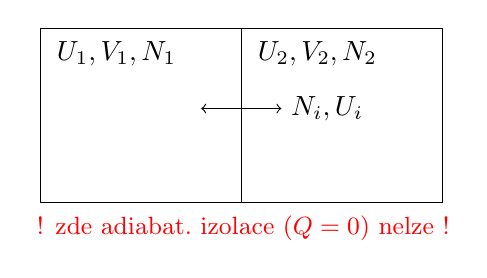
\begin{tikzpicture}[scale=0.85]
  \draw (0,0) rectangle (6,2.6);
  \draw (3,0) -- (3,2.6);
  \node[anchor=north west] at (0.1,2.55) {$U_1,V_1,N_1$};
  \node[anchor=north west] at (3.1,2.55) {$U_2,V_2,N_2$};
  \draw[<->] (2.4,1.4) -- (3.6,1.4);
  \node[right] at (3.6,1.4) {$\dd N_i,\dd U_i$};
  \node[Red,anchor=north west] at (-0.2,-0.05) {\small ! zde adiabat.\ izolace ($\dd Q = 0$) nelze !};
\end{tikzpicture}
\end{minipage}
\begin{minipage}{0.53\textwidth}
\[
  \Rightarrow\ \dd S = \sum_i\left[\left(\pdv{S_i}{U_i}\right)\dd U_i + \left(\pdv{S_i}{N_i}\right)\dd N_i\right]
\]
\[
  \dd U_1 = -\dd U_2\,, \qquad \dd N_1 = -\dd N_2
\]
\end{minipage}

\[
  \Rightarrow\quad \frac{1}{T_1} = \frac{1}{T_2}
  \quad\&\quad
  \left(\pdv{S_1}{N_1}\right)_{U_1,V_1} = \left(\pdv{S_2}{N_2}\right)_{U_2,V_2}
  \ \Leftrightarrow\ \frac{\mu_1}{T_1} = \frac{\mu_2}{T_2}
\]

\begin{minipage}{0.38\textwidth}
\begin{definice}[Chemický potenciál]
\[ \Rightarrow\ \vzorec{\left(\pdv{S}{N}\right)_{U,V} \equiv -\frac{\mu}{T}} \]
\end{definice}
\end{minipage}\hfill
\begin{minipage}{0.6\textwidth}
\textcolor{Red}{\scriptsize\itshape Závěr: \\
$\to$ podmínky stability $\dd S = 0$ mají smysl jen pro složený systém, kde jsou k dispozici nefixované vnitřní proměnné; tyto ve skutečnosti ani nemusí být extenzivní, opravdu hledáme extrém $S$ na vhodně parametrizovaném dostupném podprostoru stavového prostoru \\
$\to$ z hlediska fundamentální rovnice jednoduchého systému vedou k interpretaci derivací $S$ v termínech intenzivních proměnných -- rovnovážný stav takového systému je tak zakódován ve stavových rovnicích typu $y/T = y/T(U, X\_1,\dots,X\_k)$ \\
$\to$ detailně to uvidíme při studiu fázového přechodu ve vdW plynu -- tam $p = p(v,T)$ nemá jednoznačnou inverzi $v = v(p,T)$; různá řešení této inverze dávají různé stavové rovnice odpovídající různým fázím (kapalina, plyn); existence více stavových rovnic souvisí s existencí oblastí nestability (konvexní $S$) ve stavovém prostoru}
\end{minipage}

\textcolor{NavyBlue}{\small tady to chce stoichiometrické koef.! \quad
$2\mathrm{H}_2 + \mathrm{O}_2 \rightleftarrows 2\mathrm{H}_2\mathrm{O} \Leftrightarrow 0 \leftrightarrows \sum\nu_jA_j$ \ \&
$S = S(U,V,N_{\mathrm{H}_2},N_{\mathrm{O}_2},N_{\mathrm{H}_2\mathrm{O}})$ \\
\hspace*{5cm} $\Rightarrow \dd S = -\frac{\dd\tilde N}{T}\sum\mu_j\nu_j = 0 \Leftrightarrow \sum\mu_j\nu_j = 0$}

\begin{veta}[Obecně]
\[
  \dd S = \frac1T\dd U - \sum_i\frac{y_i}{T}\dd X_i \quad\Leftrightarrow\quad \vzorec{\dd U = T\,\dd S + \sum_i y_i\,\dd X_i}
\]
\[
  \Leftrightarrow\quad \vzorec{\left(\pdv{S}{X_i}\right)_{U,X_{j\neq i}} \equiv -\frac1T y_i}
\]
\textcolor{NavyBlue}{V rovnováze nastává rovnost mezi těmi int.\ proměnnými, které jsou sdružené s ext.\ proměnnými zprostředkujícími interakci.}
\end{veta}

%----------------------------------------------------------------------
\strana{L04b-4}
\underline{Pozn:}
\begin{itemize}
  \item $\dd U = T\dd S$ $\Rightarrow$ abs.\ \kw{teplota} je \underline{definována} jako \underline{rychlost změny energie se změnou entropie}
  \begin{itemize}[nosep]
    \item[$\to$] dosud nejobecnější definice
    \item[$\to$] je svázána s mikroskop.\ energií částic, ale není přímočaře mírou kin.\ energie jako v kinet.\ teorii \\
    (srov.\ ekvipart.\ teorém $\langle\varepsilon_k\rangle\sim\frac{f}{2}k_BT$ \textcolor{NavyBlue}{\small $\leftarrow f$ = počet kvadr.\ st.\ volnosti} vs.\ fotonový plyn (černé těleso) $U\propto T^4$)
    \item[$\to$] $S = k_B\log W$ \quad $\Rightarrow$ \quad $\vzorec{\dfrac1T = \dfrac{k_B}{W}\left(\pdv{W}{U}\right)_{V,N}}$ \\[3pt]
    $\Rightarrow$ teplota měří poměrnou změnu počtu mikrostavů se změnou $U$, nemá tedy přímý vztah k mikroskop.\ vlastnostem částic\pozor{!}
  \end{itemize}
  \item \underline{měření teploty a fluktuace} -- abychom mohli systému přiřadit teplotu, musí být schopen vyměňovat energii s okolím $\Rightarrow$ $U$ nemůže být určena s lib.\ přesností
  \begin{itemize}[nosep]
    \item[$\to$] podobně to platí pro ostatní \underline{sdružené veličiny} ($p$--$V$, $\mu$--$N$, \dots)
    \item[$\to$] rovn.\ TD ovšem fluktuace nepopisuje
  \end{itemize}
\end{itemize}

\subsection*{Stavové rovnice}
\textcolor{NavyBlue}{$\Rightarrow\ \frac1T = \frac1T(U,X_1,\dots,X_n)$, \quad $y_i = y_i(U,X_1,\dots,X_n)$}
\[
  \frac1T = \left(\pdv{S}{U}\right)_{X_j}, \qquad -\frac{y_i}{T} = \left(\pdv{S}{X_i}\right)_{U,X_{j\neq i}}
  \qquad\dots\ \text{\kw{stavové rovnice} v \underline{entropické reprezentaci}}
\]
\begin{definice}[Stavové rovnice]
$\Rightarrow$ stavové rovnice jsou \underline{závislosti intenzivních veličin na nezávislých extenzivních}
\end{definice}

\begin{itemize}
  \item \underline{energetická reprezentace} \quad \dots\ $U = U(S,X_1,\dots,X_n)$ je také \underline{fund.\ rovnice}
  \[
    \vzorec{T = \left(\pdv{U}{S}\right)_{X_j}}\,; \qquad \vzorec{y_i = \left(\pdv{U}{X_i}\right)_{S,X_{j\neq i}}}
  \]
\end{itemize}

%----------------------------------------------------------------------
\strana{L04b-5}
\begin{itemize}[nosep]
  \item[$\to$] stavové rovnice lze derivováním odvodit z \underline{fundamentální rovnice} $\Rightarrow$ tato obsahuje veškerou informaci o systému
  \item FR odvozujeme ze stav.\ rovnic ($\Leftarrow$ experiment, model) nebo ze stat.\ fyziky ($\Leftarrow\mathcal{H}$, tj.\ také model)
\end{itemize}

\underline{Pozn:} \pozor{derivace $U$ nebo $S$ mají zmíněný význam pouze tehdy, pokud derivujeme fundamentální rovnici!}

\begin{priklad}[Př:]
\begin{enumerate}[label=\roman*)]
  \item $\left(\pdv{U}{S}\right)_{V,N} = T$ \quad \textcolor{NavyBlue}{$\Leftarrow U = U(S,V,N)$}
  \item
  \begin{align*}
    \left(\pdv{U}{S}\right)_{\textcolor{Red}{p},N}
      &= \left(\frac{\partial U(S,p,N)}{\partial S}\right) = \Big/\,V = V(S,p,N)\,\Big/ =
       \frac{\partial U\big(S, V(S,p,N), N\big)}{\partial S} \\
      &= \left(\pdv{U}{S}\right)_{V,N} + \left(\pdv{U}{V}\right)_{S,N}\left(\pdv{V}{S}\right)_{p,N} \\
      &= T - p\left(\pdv{V}{S}\right)_{p,N}
       = \Big/\,\begin{array}{l}\text{trajektorii } (p = \text{konst}, N = \text{konst}) \\ \text{parametrizuji teplotou} \Rightarrow V = V(T),\ S = S(T)\end{array}\Big/ \\
      &= T - p\left(\pdv{V}{T}\right)_{p,N}\left(\pdv{T}{S}\right)_{p,N}
       = T - pVT\,\frac{\frac1V\left(\pdv{V}{T}\right)_{p,N}}{T\left(\pdv{S}{T}\right)_{p,N}}
  \end{align*}
  \[
    \Rightarrow\ \vzorec{\left(\pdv{U}{S}\right)_{p,N} = T\left(1 - \frac{pV\alpha}{C_p}\right)}
    \qquad
    \alpha = \frac1V\left(\pdv{V}{T}\right)_p
  \]
  \dots\ \kw{koeficient tepelné roztažnosti}
\end{enumerate}
\end{priklad}

\underline{Pozn:} $\bullet$ důsledky analytické struktury termodyn.\ funkcí:
\[
  \alpha = \frac1V\left(\pdv{V}{T}\right)_p\,;\qquad \kappa_T = -\frac1V\left(\pdv{V}{p}\right)_T
  \qquad\qquad \left(\pdv{p}{T}\right)_V = \;? \ \text{ je to nezávislá veličina?}
\]
\pozor{NE!} \ pravidlo $-1$:
\[
  \left(\pdv{V}{T}\right)_p\left(\pdv{T}{p}\right)_V\left(\pdv{p}{V}\right)_T = -1
  \quad\Rightarrow\quad
  \vzorec{\left(\pdv{p}{T}\right)_V = -\frac{(\partial V/\partial T)_p}{(\partial V/\partial p)_T} = \frac{\alpha}{\kappa_T}}
\]

%----------------------------------------------------------------------
\strana{L04b-6}
\subsection{Extenzivita entropie}
\subsubsection*{1) Eulerova rovnice}
Eulerův teorém: \quad $F(\lambda X_1,\dots,\lambda X_n) = \lambda^pF(X_1,\dots,X_n)$ \quad (homog.\ fce $p$-tého řádu) $\Rightarrow$
\[
  p\lambda^{p-1}F(X_1,\dots,X_n) = \sum_i\left(\frac{\partial F}{\partial(\lambda X_i)}\right)\left(\frac{\partial(\lambda X_i)}{\partial\lambda}\right)
  = \sum_i X_i\frac{\partial F}{\partial Y_i}(Y_1,\dots,Y_n)\Big/_{Y_i = \lambda X_i}
\]
\[
  \overset{\lambda = 1}{\Rightarrow}\qquad \vzorec{pF(X_1,\dots,X_n) = \sum_i X_i\pdv{F}{X_i}}
\]
\begin{itemize}
  \item entropie je homog.\ funkce 1.\ řádu ($p = 1$)
\end{itemize}
\begin{veta}[Eulerova rovnice]
\[
  \vzorec{TS = U - \sum_i y_iX_i = U + pV - \mu N}
\]
\end{veta}
\begin{itemize}
  \item $T, y_i$ je ovšem třeba chápat jako funkce extenzivních proměnných:
  \[
    U(S,V,N) = T(S,V,N)\,S - p(S,V,N)\,V + \mu(S,V,N)\,N
  \]
  $\to$ stejně pro $S(U,V,N)$
  \item z Eulerovy rovnice ihned plyne intenzivnost teploty a dalších derivací entropie/energie
\end{itemize}

\subsubsection*{2) Gibbsův--Duhemův vztah}
\begin{itemize}[nosep]
  \item diferenciál ER $\Rightarrow$ \quad
  $T\,\cancel{\dd S} + S\,\dd T = \cancel{\dd U} + \cancel{p\,\dd V} + V\dd p - \cancel{\mu\,\dd N} - N\dd\mu$
  \item diferenciál $U$ $\Rightarrow$ \quad $\dd U = T\dd S - p\dd V + \mu\dd N$
\end{itemize}
\begin{veta}[Gibbsův--Duhemův vztah]
\[
  \Rightarrow\ \vzorec{\dd\mu = -s\,\dd T + v\,\dd p} \qquad s\equiv\frac{S}{N}\ \ \&\ \ v\equiv\frac{V}{N}
  \qquad\Rightarrow\ \mu = \mu(T,p)
\]
\end{veta}
\begin{itemize}
  \item Eulerova rovnice resp.\ G-D vztah je to, co nám umožňuje integrovat fundamentální rovnici bez znalosti chem.\ potenciálu:
  \begin{enumerate}[label=\arabic*)]
    \item $s = s(u,v)$ $\leftrightarrow$ $\dd s = \dfrac{\dd u}{T} + \dfrac{p}{T}\dd v$
    \item $\begin{cases}
            \to\ S(U,V,N) = N\,s\!\left(\frac{U}{N},\frac{V}{N}\right) \\
            \to\ \text{G-D}\ \to\ \mu(s,v)\ \to\ \mu(u,v)\ \to\ TS = U + pV - \mu N
          \end{cases}$
  \end{enumerate}
\end{itemize}

%----------------------------------------------------------------------
\strana{L04b-7}
\begin{itemize}
  \item jinak řečeno, změna $\mu$ není nezávislá, je určena změnami $T$ a $p$ \\
  $\Rightarrow$ ačkoliv je stav systému specifikován 3 extenzivními parametry, jen 2 ze 3 odpovídajících intenzivních jsou nezávislé $\Rightarrow$ k úplné specifikaci stavu systému potřebujeme vždy alesp.\ 1 extenzivní veličinu
  \item \underline{zobecnění na $l$ chem.\ komponent:}
\end{itemize}
\begin{veta}[Euler a G-D pro $l$ komponent]
\[
  \begin{aligned}
    TS &= U + pV - \sum_{j=1}^{l}\mu_jN_j &&\qquad\text{EULER} \\
    \sum_{j=1}^{l}N_j\,\dd\mu_j &= -S\,\dd T + V\,\dd p &&\qquad\text{G-D}
  \end{aligned}
\]
\end{veta}
$\Rightarrow$ systém má $l + 1$ nez.\ intenzivních parametrů \quad $\#(U,V,N_1,\dots,N_l)$ minus 1

\textcolor{Red}{\textbf{! celé je to důsledek extenzivity !}} \ \underline{platnost tedy není zcela univerzální}

\subsection*{Shrnutí}
\begin{enumerate}[label=\arabic*)]
  \item \kw{fundamentální (FR) rovnice} obsahuje veškerou TD informaci \\
  \quad $S = S(U,V,N)$ \ nebo \ $U = U(S,V,N)$ \qquad \textcolor{NavyBlue}{(tj.\ stav.\ rovnice, určuje rovn.\ stavy)}
  \item stavové rovnice dostáváme derivováním:
  \[
    T = \left(\pdv{U}{S}\right)_{V,N} \qquad -p = \left(\pdv{U}{V}\right)_{S,N} \qquad \mu = \left(\pdv{U}{N}\right)_{S,V}
  \]
  -- tyto 3 jsou pro jednokomponentní systém ekvivalentní znalosti FR \textcolor{NavyBlue}{(pro ext.\ syst.\ např.\ skrze Eulerovu rovnici)}
  \item pro extenzivní systém jsou stav.\ rovnice svázány G-D relací
  \[
    \dd\mu = -s\,\dd T + v\,\dd p
  \]
  \textcolor{NavyBlue}{$\Rightarrow$ stačí 2 stav.\ rovnice, ovšem dostávám $\tilde\mu = \mu + \mu_0$ ($\mu_0$ je integ.\ konst.) \\
  $\Rightarrow U = TS - pV + \mu N \textcolor{Red}{{}+\mu_0N}$ \dots\ o trochu méně než znám-li stav.\ rci pro $\mu$ bez volného $\mu_0$}
  \item $U(T,V,N)$, $U(S,p,N)$ \underline{nejsou} FR \\
  -- ve skutečnosti se jedná o parciální dif.\ rovnice:
  \[
    U(T,V,N) = U\!\left(\pdv{U}{S}, V, N\right)
  \]
  (viz přednáška Termodynamické potenciály)
\end{enumerate}

%----------------------------------------------------------------------
\strana{L04b-8}

\begin{center}
\begin{tikzpicture}[scale=1.0,>=Stealth]
  % osy
  \draw[->] (0,0) -- (0,4) node[left] {$S$};
  \draw[->] (0,0) -- (-3,0) node[above] {$U$};
  \draw[->] (0,0) -- (4.5,-3) node[below] {$X_j$};
  % rovina S = S0
  \draw[OliveGreen,dotted,thick] (-2.3,2.4) -- (0,2.4) -- (6.4,-1.8) -- (4,-1.8);
  \node[OliveGreen] at (-1.3,2) {$S = S_0$};
  % nadplocha
  \draw[thick] (0.7,-2.9) .. controls (0.3,-1) and (0.5,1.5) .. (1.3,2.7)
               .. controls (2,3.3) and (2.6,3.1) .. (3.1,2.9)
               .. controls (3.7,2.5) and (3.9,0.5) .. (3.6,-1.4)
               .. controls (3.5,-2.6) and (2.4,-3.1) .. (0.7,-2.9);
  \draw[thick,dashed] (3.1,2.9) .. controls (2.3,1.5) and (2,-0.5) .. (1.4,-1.5)
                       .. controls (1,-2.2) .. (0.7,-2.9);
  % červená křivka (vratný kvazistatický proces)
  \draw[Red,thick,dashed] (0.9,0.6) .. controls (1.2,1.2) and (1.6,1.5) .. (2,1.6);
  \draw[Red,thick] (0.9,0.6) .. controls (1.3,-0.2) and (2,-0.3) .. (2.6,-0.3)
                   .. controls (3,-0.3) and (3.5,-0.1) .. (3.8,0.2);
  \fill[Red] (0.9,0.6) circle (2pt) node[left] {B};
  \fill[Red] (1.45,1.25) circle (2pt) node[above left] {A};
  \fill[Red] (2,1.6) circle (2pt);
  \fill[Red] (2.2,-0.25) circle (2pt) node[below] {C};
  \fill[Red] (3.8,0.2) circle (2pt) node[right] {D};
  % modrá křivka (nevratný kvazistatický)
  \draw[NavyBlue,thick] (1.3,-2.3) .. controls (1.4,-1) and (2.3,-0.8) .. (2.4,0.3)
                        .. controls (2.5,1.2) and (2.6,1.8) .. (2.9,1.9);
  \fill[NavyBlue] (1.3,-2.3) circle (2pt) (2.9,1.9) circle (2pt);
  \draw[NavyBlue,->] (1.6,-2.4) -- (1.6,-1.7);
  \node[NavyBlue,font=\small,align=left] at (2.4,-2.2) {uvolňuji\\omezení};
  % popisky
  \draw[NavyBlue,->] (4.6,3.6) .. controls (2.4,3.6) .. (2.3,3.15);
  \node[NavyBlue,font=\small,align=left,anchor=west] at (4.6,3.6) {$S = S(U,X_1,\dots,X_n)$ -- každý bod nadplochy\\odpovídá rovnovážnému stavu};
  \draw[NavyBlue,->] (5.3,1.8) -- (2.55,1.3);
  \node[NavyBlue,font=\small,align=left,anchor=west] at (5.3,1.95) {\underline{nevratný} \underline{(rovnovážný) kvazistatický} děj};
  \draw[Red,->] (-1.5,-1.2) -- (0.8,0.1);
  \node[Red,font=\small,align=left] at (-2,-1.7) {\underline{vratný kvazistat.}\\proces:\\$S(U,X_j) = S_0$};
\end{tikzpicture}
\end{center}

\textcolor{NavyBlue}{
\begin{enumerate}[label=\roman*),nosep]
  \item nevratný: \ $\dd S > 0$
  \item kvazistatický: \\
  $\to$ probíhá po povrchu nadplochy \\
  $\to$ $\dd S = \frac1T\dd U - \sum_j\frac{y_j}{T}\dd X_j$ \\
  (pro nekvazistac.\ identifikace $\frac1T = \left(\pdv{S}{U}\right)_{X_j}$ etc.\ neplatí!, resp.\ $S$ není def.!)
\end{enumerate}}

\textcolor{Red}{
\begin{itemize}[nosep]
  \item[$\to$] vratný proces je vždy kvazistatický -- je to limita kvazistatického procesu s $\dd S = 0$
  \item[$\to$] vratný proces nemůže být nerovnovážný:
  \begin{itemize}[nosep]
    \item relaxace -- přechod z nerovnovážného stavu do rovnováhy -- je nutně nevratný, $\Delta S > 0$; kdyby byl vratný, mohl by systém rovnováhu opustit zpět k nerovnováze \underline{samovolně}
  \end{itemize}
\end{itemize}}

